%%%%%%%%%%%%%%%%%%%%%%%%
%
% $Autor: Sadegh Naderi $
% $Datum: 2023-11-24  $
% $Short Description: Explanation about how to test the code $
% $Directory: ML23-01-Keyword-Spotting-with-an-Arduino-Nano-33-BLE-Sense\report\Contents\en\testSoftware.tex $
% $Version: 2.0 $
%
%%%%%%%%%%%%%%%%%%%%%%%%


\chapter{Software Tests}
\label{chapter:SoftwareTests}


\section{Introduction}

One of the principles of \textbf{agile} development (although not exactly being the case for our study) is that testing should be tightly integrated with development, and programmers should write tests for their own code \cite{Ousterhout:2018}.

\begin{itemize}
	\item unit tests
	\begin{itemize}
		\item most often written by developers
		\item small and focused
		\item are often run in conjunction with a test coverage tool\footnote{ensures that every line of code in the application is tested.}
		\begin{itemize}
			\item Coverage.py
			\item pytest-cov
		\end{itemize}
	\end{itemize}
\end{itemize}

When writing new code or modifying existing code, it is essential to update the corresponding unit tests to ensure continued code functionality and test coverage \cite{Ousterhout:2018}.

Unit tests facilitate refactoring \cite{Ousterhout:2018}. Without a test suite

\begin{itemize}
	\item It would be dangerous to make major structural changes to a system.
	\item bugs will go undetected until the new code is deployed.
	\begin{itemize}
		\item much more expensive to find and fix
	\end{itemize}
\end{itemize}

With a good set of tests, developers can be more confident when refactoring because the test suite will find most bugs that are introduced \cite{Ousterhout:2018}. 


\section{"Hello World" Example: How to test Python files}

In this section, an example of testing Python files using a simple "Hello World" calculator module is provided. The example consists of two files: \texttt{calc.py} (the calculator module) and \texttt{testCalc.py} (the unit test module).

\subsection{Calculator Module (\texttt{calc.py})}

The \texttt{calc.py} file contains a basic calculator module with an addition function (see Listing \ref{code:calc}).

\begin{code}[h!]
	\lstinputlisting[language=Python, numbers=none, linerange={56-65}]{Code/testExample/calc.py}    
	
	\caption{Calculator Module (\texttt{calc.py})}
	\label{code:calc}
\end{code}

The \texttt{calc.py} module provides a simple \texttt{addition} function, allowing users to perform addition operations. This function will be tested in the subsequent unit test module.

\subsection{Unit Test Module (\texttt{testCalc.py})}

The \texttt{testCalc.py} file contains unit tests for the functions in the `calc` module. The primary test case, \texttt{TestCalc.test\_addition}, checks the correctness of the \texttt{addition} function. Below is the relevant portion of the code:

\begin{code}[h!]
	\lstinputlisting[language=Python, numbers=none, linerange={24-41}]{Code/testExample/testCalc.py}    
	
	\caption{Unit Test Module (\texttt{testCalc.py})}
	\label{code:testCalc}
\end{code}

The unit tests include cases with positive integers (5, 5) and mixed integers (-1, 1), with the expected results of 10 and 0, respectively.

\subsection{Run the Test with \texttt{pytest}}

To run the tests and for automation purposes, \texttt{pytest} package (explained in the section \ref{subsection:pytest}) is used.

Open the command prompt or terminal and navigate to the directory where your project and test files are located.

In the command prompt or terminal, simply run the following command to execute your test:

\begin{verbatim}
	pytest
\end{verbatim}

This will discover and run all the tests in your project.

\textbf{Note:} To be able to run the pytest command, the name of the file \texttt{testCalc.py} should be changed to \texttt{test\_calc.py} so that pytest would automatically recognize the file as a test file.

The result is shown in Figure \ref{fig:pytestExampleResult}. The output from \texttt{pytest} indicates that one test item (test file) was collected.

\begin{verbatim}
	collected 1 item
\end{verbatim}

This green line summarizes the test results. It states that one test passed, and it took 0.08 seconds to run.

\begin{verbatim}
	1 passed in 0.08s
\end{verbatim}


\begin{figure}[h!]
	\centering
	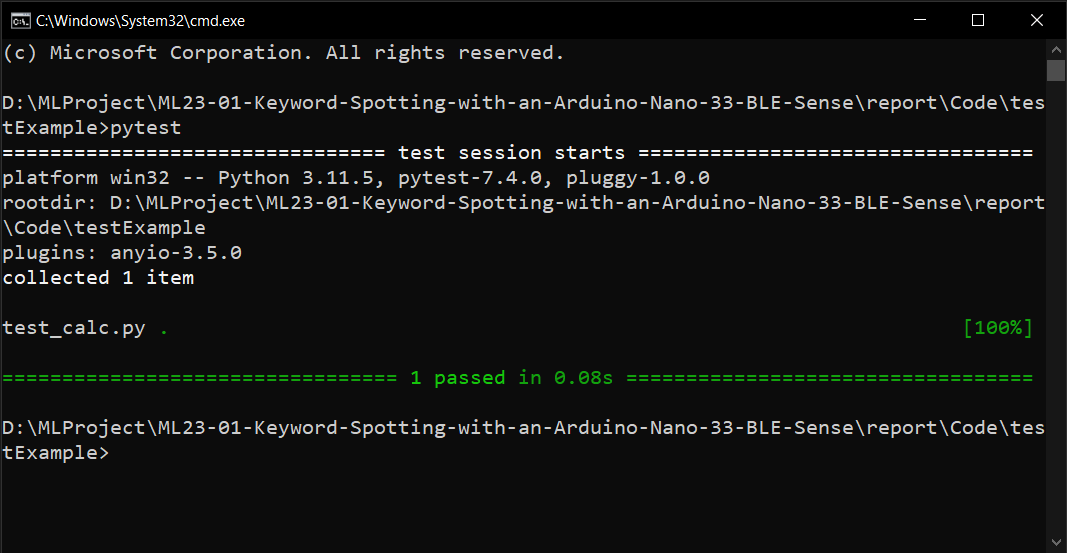
\includegraphics[width=0.8\textwidth]{Images/testSoftware/pytestExampleResult}
	\caption{Result of running \texttt{pytest} in the direcotry of the test file in \texttt{Command Prompt}} 
	\label{fig:pytestExampleResult}
\end{figure}


\section{Test Files}



\begin{itemize}
	\item The \texttt{unittest.main()} block at the end of each script ensures that the unit tests are executed when the script is run as the main program.
	\item Each script contains specific test cases checking functionalities within their respective modules (\texttt{dataUtils}, \texttt{modelUtils}, and \texttt{exportUtils}).
\end{itemize}


\subsection{\texttt{testDataUtils.py}}

\subsubsection{File Overview}

\begin{itemize}
	\item \textbf{Purpose:}
	\begin{itemize}
		\item This script serves as a unit test suite for the \texttt{dataUtils} module.
		\item It contains individual test cases to verify the functionality of key functions related to loading, preprocessing, and creating spectrogram datasets from audio data.
	\end{itemize}
\end{itemize}

\subsubsection{Test Cases}

\textbf{\PYTHON{testLoadDataset}}

\begin{itemize}
	\item \textbf{Objective:} Checks if the \texttt{loadDataset} function successfully loads audio datasets.
	\item \textbf{Testing Approach:}
	\begin{itemize}
		\item Calls \texttt{loadDataset} with specified parameters.
		\item Asserts that the returned objects are instances of TensorFlow datasets (\texttt{tf.data.Dataset}).
	\end{itemize}
\end{itemize}

\begin{code}[h!]
	\lstinputlisting[language=Python, numbers=none, linerange={35-44}]{../Code/KeywordSpotting/testDataUtils.py}
	
	\caption{The \PYTHON{testLoadDataset} method}
	\label{code:testLoadDataset}
\end{code}

\textbf{\texttt{testPreprocessAudioDataset}}

\begin{itemize}
	\item \textbf{Objective:} Checks if the \texttt{preprocessAudioDataset} function successfully preprocesses audio datasets.
	\item \textbf{Testing Approach:}
	\begin{itemize}
		\item Creates a mock dataset.
		\item Calls \texttt{preprocessAudioDataset} with the mock dataset.
	\end{itemize}
\end{itemize}

\begin{code}[h!]
	\lstinputlisting[language=Python, numbers=none, linerange={46-53}]{../Code/KeywordSpotting/testDataUtils.py}
	
	\caption{The \PYTHON{testPreprocessAudioDataset} method}
	\label{code:testPreprocessAudioDataset}
\end{code}

\textbf{\texttt{testCreateSpectrogramDataset}}

\begin{itemize}
	\item \textbf{Objective:} Checks if the \texttt{createSpectrogramDataset} function successfully creates spectrogram datasets.
	\item \textbf{Testing Approach:}
	\begin{itemize}
		\item Creates a mock dataset with preprocessed audio data.
		\item Calls \texttt{createSpectrogramDataset} with the mock dataset.
	\end{itemize}
\end{itemize}

\begin{code}[h!]
	\lstinputlisting[language=Python, numbers=none, linerange={55-72}]{../Code/KeywordSpotting/testDataUtils.py}
	
	\caption{The \PYTHON{testCreateSpectrogramDataset} method}
	\label{code:testCreateSpectrogramDataset}
\end{code}


This test script is a component of a testing strategy, ensuring that the functions in the \texttt{dataUtils} module, encapsulated within the \texttt{TestDataUtils} class, perform as expected.

\begin{code}[h!]
	\lstinputlisting[language=Python, numbers=none, linerange={29}]{../Code/KeywordSpotting/testDataUtils.py}
	
	\caption{The \PYTHON{TestDataUtils} class}
	\label{code:TestDataUtils}
\end{code}


\subsection{\texttt{testModelUtils.py}}

\subsubsection{File Overview}

\begin{itemize}
	\item \textbf{Purpose:}
	\begin{itemize}
		\item This script serves as a unit test suite for the \texttt{modelUtils} module.
		\item It includes tests for building a model using the \texttt{buildModel} function.
	\end{itemize}
\end{itemize}

\subsubsection{Test Cases}

\textbf{\texttt{testBuildModel}}

\begin{itemize}
	\item \textbf{Objective:} Checks if the \texttt{buildModel} function successfully constructs a model.
	\item \textbf{Testing Approach:}
	\begin{itemize}
		\item Calls \texttt{buildModel} with specified parameters.
		\item Asserts that the returned model is an instance of \texttt{tf.keras.models.Sequential}.
		\item Checks each layer in the model against the expected structure.
	\end{itemize}
\end{itemize}


\begin{code}
	\lstinputlisting[language=Python, numbers=none, linerange={38-77}]{../Code/KeywordSpotting/testModelUtilst.py}
	
	\caption{The \PYTHON{testBuildModel} method}
	\label{code:testBuildModel}
\end{code}

This test script is designed to ensure that the \texttt{modelUtils} module's \texttt{buildModel} function constructs models with the expected structure. The \texttt{testBuildModel} function is defined inside the \texttt{TestModelUtils} class. 

\begin{code}[h!]
	\lstinputlisting[language=Python, numbers=none, linerange={31}]{../Code/KeywordSpotting/testModelUtilst.py}
	
	\caption{The \PYTHON{TestModelUtils} class}
	\label{code:TestModelUtils}
\end{code}

\subsection{\texttt{testExportUtils.py}}

\subsubsection{File Overview}

\begin{itemize}
	\item \textbf{Purpose:}
	\begin{itemize}
		\item This script serves as a unit test suite for the \texttt{exportUtils} module.
		\item It includes tests for exporting a model, saving a model, and converting a model to TFLite format.
	\end{itemize}
\end{itemize}

\subsubsection{Test Cases}

\textbf{\texttt{TestExportUtils} Class}

\begin{itemize}
	\item \textbf{\texttt{testExportModel}}
	\begin{itemize}
		\item \textbf{Objective:} Checks if the \texttt{ExportModel} class in the \texttt{exportUtils} module is functioning correctly.
		\item \textbf{Testing Approach:}
		\begin{itemize}
			\item Creates a mock \texttt{Sequential} model and label names.
			\item Instantiates an \texttt{ExportModel} instance and asserts that it is created without errors.
		\end{itemize}
	\end{itemize}
	
	\item \textbf{\texttt{testSaveModel}}
	\begin{itemize}
		\item \textbf{Objective:} Checks if the \texttt{saveModel} function in the \texttt{exportUtils} module successfully saves a model.
		\item \textbf{Testing Approach:}
		\begin{itemize}
			\item Creates a mock \texttt{Sequential} model.
			\item Calls \texttt{saveModel} with the model and a specified save path.
			\item Asserts that the save directory is created and, optionally, checks for specific files or conditions within the directory.
			\item Cleans up by removing the save directory after the test.
		\end{itemize}
	\end{itemize}
	
	\item \textbf{\texttt{testConvertToTFLite}}
	\begin{itemize}
		\item \textbf{Objective:} Checks if the \texttt{convertToTFLite} function in the \texttt{exportUtils} module handles exceptions during the conversion process.
		\item \textbf{Testing Approach:}
		\begin{itemize}
			\item Uses \texttt{self.assertRaises} to check if an exception is raised when calling \texttt{convertToTFLite} with specified parameters.
		\end{itemize}
	\end{itemize}
\end{itemize}

\begin{code}[h!]
	\lstinputlisting[language=Python, numbers=none, linerange={41-51}]{../Code/KeywordSpotting/testExportUtils.py}
	
	\caption{The \PYTHON{testExportModel} method}
	\label{code:testExportModel}
\end{code}

\begin{code}[h!]
	\lstinputlisting[language=Python, numbers=none, linerange={53-71}]{../Code/KeywordSpotting/testExportUtils.py}
	
	\caption{The \PYTHON{testSaveModel} method}
	\label{code:testSaveModel}
\end{code}

\begin{code}
	\lstinputlisting[language=Python, numbers=none, linerange={73-82}]{../Code/KeywordSpotting/testExportUtils.py}
	
	\caption{The \PYTHON{testConvertToTFLite} method}
	\label{code:testConvertToTFLite}
\end{code}

This test script is part of the testing strategy, ensuring the correct functionality of the \texttt{exportUtils} module's key features, encapsulated within the \texttt{TestExportUtils} class.

\begin{code}[h!]
	\lstinputlisting[language=Python, numbers=none, linerange={31}]{../Code/KeywordSpotting/testExportUtils.py}
	
	\caption{The \PYTHON{TestExportUtils} class}
	\label{code:TestExportUtils}
\end{code}


\section{Automation}

To automate the testing process, the pytest package is used.

\subsection{pytest}
\label{subsection:pytest}

\subsubsection{Installing \texttt{Pytest}}

You can install \texttt{pytest} using pip:

\begin{verbatim}
	pip install pytest
\end{verbatim}

\subsubsection{Writing Test Functions}

Create a Python file for your tests, and name it with a \texttt{test\_} prefix (e.g., \texttt{test\_my\_code.py}). Write test functions with names starting with \texttt{test\_}:

\begin{lstlisting}[language=Python, numbers=none]
	# test_myCode.py
	
	def test_addition():
	assert 1 + 1 == 2
	
	def test_subtraction():
	assert 3 - 1 == 2
\end{lstlisting}

\subsubsection{Running Tests}

Run pytest from the command line, specifying the test file:

\begin{verbatim}
	pytest test_myCode.py
\end{verbatim}


\subsubsection{Test Assertions}

Use \texttt{assert} statements to check conditions. If the condition is False, pytest will raise an exception, and the test will fail:

\begin{lstlisting}[language=Python, numbers=none]
	def test_multiply():
	result = 2 * 3
	assert result == 6, "Multiplication failed"
\end{lstlisting}

\subsubsection{Test Fixtures}

Fixtures are a way to set up preconditions for your tests. Use the \texttt{@pytest.fixture} decorator:

\begin{lstlisting}[language=Python, numbers=none]
	import pytest
	
	@pytest.fixture
	def setup_data():
	data = {"key": "value"}
	return data
	
	def test_data_length(setup_data):
	assert len(setup_data) == 1
\end{lstlisting}

\subsubsection{Running Specific Tests}

You can run specific tests by specifying their names:

\begin{verbatim}
	pytest test_myCode.py::test_addition
\end{verbatim}


\subsubsection{Command Line Options}

\begin{itemize}
	\item \texttt{-v} or \texttt{--verbose}: Increase verbosity.
	\item \texttt{-k EXPRESSION}: Only run tests with names matching the given substring expression.
	\item \texttt{--cov=PACKAGE}: Measure code coverage.
	\item \texttt{--durations=N}: Print the N slowest tests.
\end{itemize}

\subsubsection{Plugins}

pytest has a rich ecosystem of plugins. You can discover and install them to extend pytest's functionality:

\begin{verbatim}
	pip install pytest-someplugin
	pytest --someplugin
\end{verbatim}


\subsection{Execution}

The result of running \texttt{pytest} in the \texttt{Command Prompt} in the directory of the test files is shown in Figure \ref{fig:pytestResult}.

\begin{figure}[h!]
	\centering
	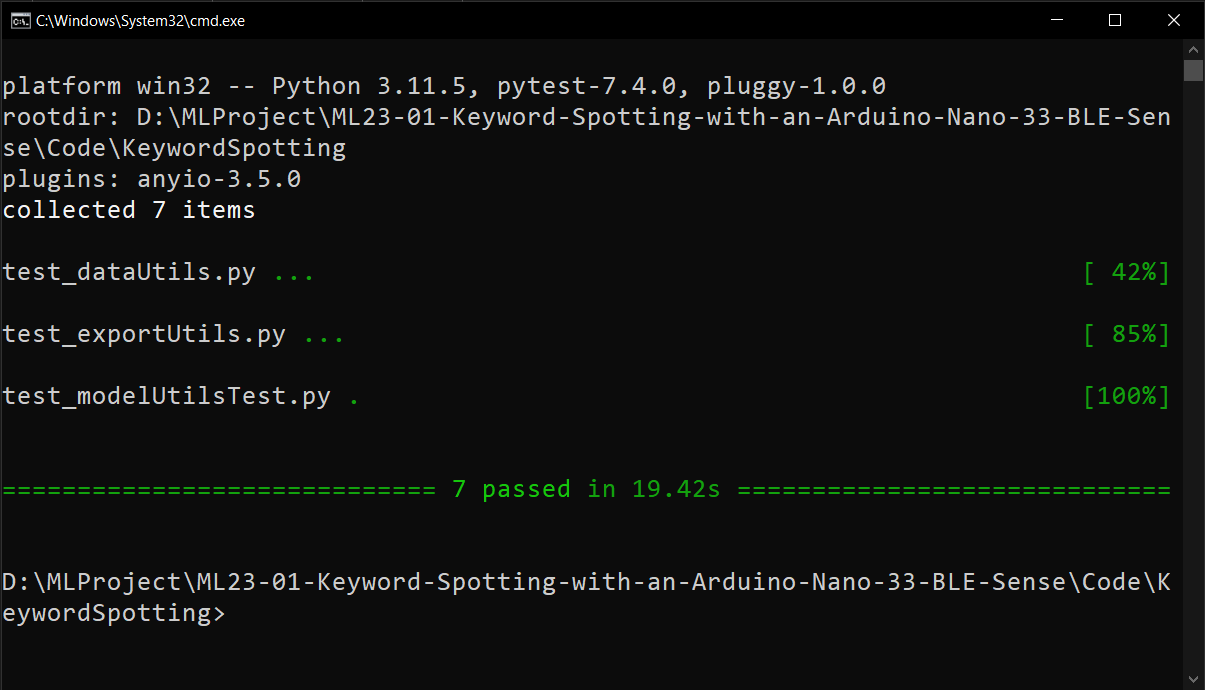
\includegraphics[width=0.8\textwidth]{Images/testSoftware/pytestResult}
	\caption{Result of running \texttt{pytest} in the direcotry of the test files in \texttt{Command Prompt}} 
	\label{fig:pytestResult}
\end{figure}

\begin{verbatim}
	collected 7 items
\end{verbatim}

This line indicates that \texttt{pytest} found and collected a total of 7 test items. These items represent individual test files or modules in the project. Note that the name of the files has been changed, starting with "\texttt{test\_}" so that \texttt{pytest} could automatically find them.

\begin{verbatim}
	test_dataUtils.py ...                      [ 42%]
	test_exportUtils.py ...                    [ 85%]
	test_modelUtilst.py .                      [100%]
\end{verbatim}

Each line corresponds to the progress of test execution for a specific test file. Dots (\texttt{...} and \texttt{.}) represent successful tests. For the case of \texttt{...}, three tests were successful, each dot representing a successful test. The percentage values ([42\%], [85\%], [100\%]) indicate the progress through the entire test suite.

\begin{verbatim}
	7 passed in 28.32s 
\end{verbatim}

This final summary line provides an overview of the test results. It states that out of the 7 tests executed, all 7 passed successfully. The total execution time for all tests was 28.32 seconds. The [100\%] success rate indicates that all the tests you ran have passed.


